\mtnote{TODO: replace `resource' with `site'; `http' to `HTTP'?}

The design of the Production and Distributed Analysis (PanDA) system started in
2005 to develop a WMS for the ATLAS experiment. PanDA went into production for
the LHC run 1 between 2009 and 2013 and was then partially redesigned to be
deployed on run 2, between 2015 and 2018. New design features are constantly
prototyped and tested on small scale but, in this section, we summarize the
design, architecture, and execution process of the current state of the
practice.

\subsection{Design}

% \begin{itemize}
%   \item Serve both individual and production workflows
%   \item hide WLCG resources behind a single interface
%   \item queue-based interface to the application layer
%   \item pilot-based
%   \item job-based
%   \item global view of the properties and states of all the jobs
%   \item global view of the available resources as a single worldwide
%      processing resource.
%   \item centralize data management
%   \item X509 AAA
%   \item Multitenancy
% \end{itemize}

\begin{itemize}
  \item No MPI tasks?
  \item Pilot multitenancy?
  \item PanDA Server Brokerage component and Event service interaction?
  \item PanDA Server Data Service component and Event Service interaction?
\end{itemize}

PanDA's application model primarily assumes tasks, as single entities or
organized into workloads or workflows. Since 2005, a certain amount of
parallelism has been progressively introduced assuming both single core and
multi-threaded tasks~\cite{multithreaded_tasks} but, so far, no MPI tasks have
been considered for production. Tasks are assumed to have at least two types of
data dependences: one or more input file and one or more data sources. Task are
also supposed to be relatively self-contained, capable of setting up their own
execution environment or having a minimal set of common dependences. Different
types of task executable are assumed, both in terms of user-defined batch
scripts or application frameworks for group of users.

PanDA's user model is based on multitenancy and the support of at least two
types of HEP users: individual researchers and groups executing production-grade
workflows. Users are considered free to submit tasks and workflows at any point
in time, directly or via dedicated application frameworks. Consistently, PanDA's
security model is based on separation between authentication, authorization and
accounting for both single users and group of users. Both authentication and
authorization are based on digital certificates and the X.509 standard.

Currently, PanDA's execution model is based on five main abstractions: task,
job, queue, pilot, and event. Tasks are assumed to be partitioned into one or
more job, possibly of variable sizes. Jobs have both attributes and states and
are queued into a global queue for execution. Prioritization and binding of jobs
are assumed to depend on the attributes of each job. Pilot abstracts resource
capabilities and jobs are bound to pilots and executed by consuming their
resources. Consistently, pilots are considered to be multitenant as jobs
belonging to multiple workflows and/or users could be bound and executed on
them.

PanDA' data model uses events as the unit of data. Each event represents a
collision captured in the detector and one or more events can be packaged into
files or data source with other abstractions. As with jobs, data have both
attributes and states and some of the attributes are linked to those of jobs so
to create an association between the two otherwise separated entities. Data are
assumed to be stored centrally, replicated when necessary and transferred over
the network. This assumptions applies to both input and output data.

PanDA design supports provenance and traceability for both jobs and data.
Attributes enable provenance by linking jobs and data items, providing
information like ownership or project affiliation. States enable traceability by
providing information about the stage of the execution in which each job or data
item is or have been. Some attributes are assumed to be immutable across
execution and jobs and data items are assumed to be always in one and only one
state.

\subsection{Architecture}

The implementation of PanDA consists of several interconnected subsystems, most
of them built from off-the-shelf and Open Source components. At a high level,
PanDA's architecture has six subsystems: PanDA Server, AutoPyFactory, PanDA
Pilot, PanDA Monitoring, JEDI, and Event Service. Subsystems communicate via
dedicated interfaces, implemented as API or http messaging. Databases are used
to store eventful entities like tasks, jobs and events, and to store information
about resources, logs, and accounting. Each subsystems is implemented as one or
more modules as shown in Figure~\ref{fig:architecture}. In the following we
briefly describe the overall architecture of PanDA and its components. The
description provides all the details required to understand how HPC resources
have been integrated within PanDA. For a full description of PanDA architecture
see~\cite{wiki, papers}.

Capabilities:
\begin{itemize}
  \item interoperable across job submission systems
  \item asynchronous distribution of input/out data organized as file collections associated to (set of) jobs.
  \item policy-aware scheduling
  \item Supporting multiple types of executable code.
\end{itemize}

% Components:
% \begin{itemize}
%   \item monitoring system
%   \item information system (static/dynamic information)
%   \item data management system
%   \item
% \end{itemize}

% \begin{itemize}
% \item PanDA Server
% \item Pilot
% \item Factory
% \item PanDA monitoring
% \item JEDI ??
% \item What else?
% \end{itemize}

\begin{figure}
  \begin{center}
    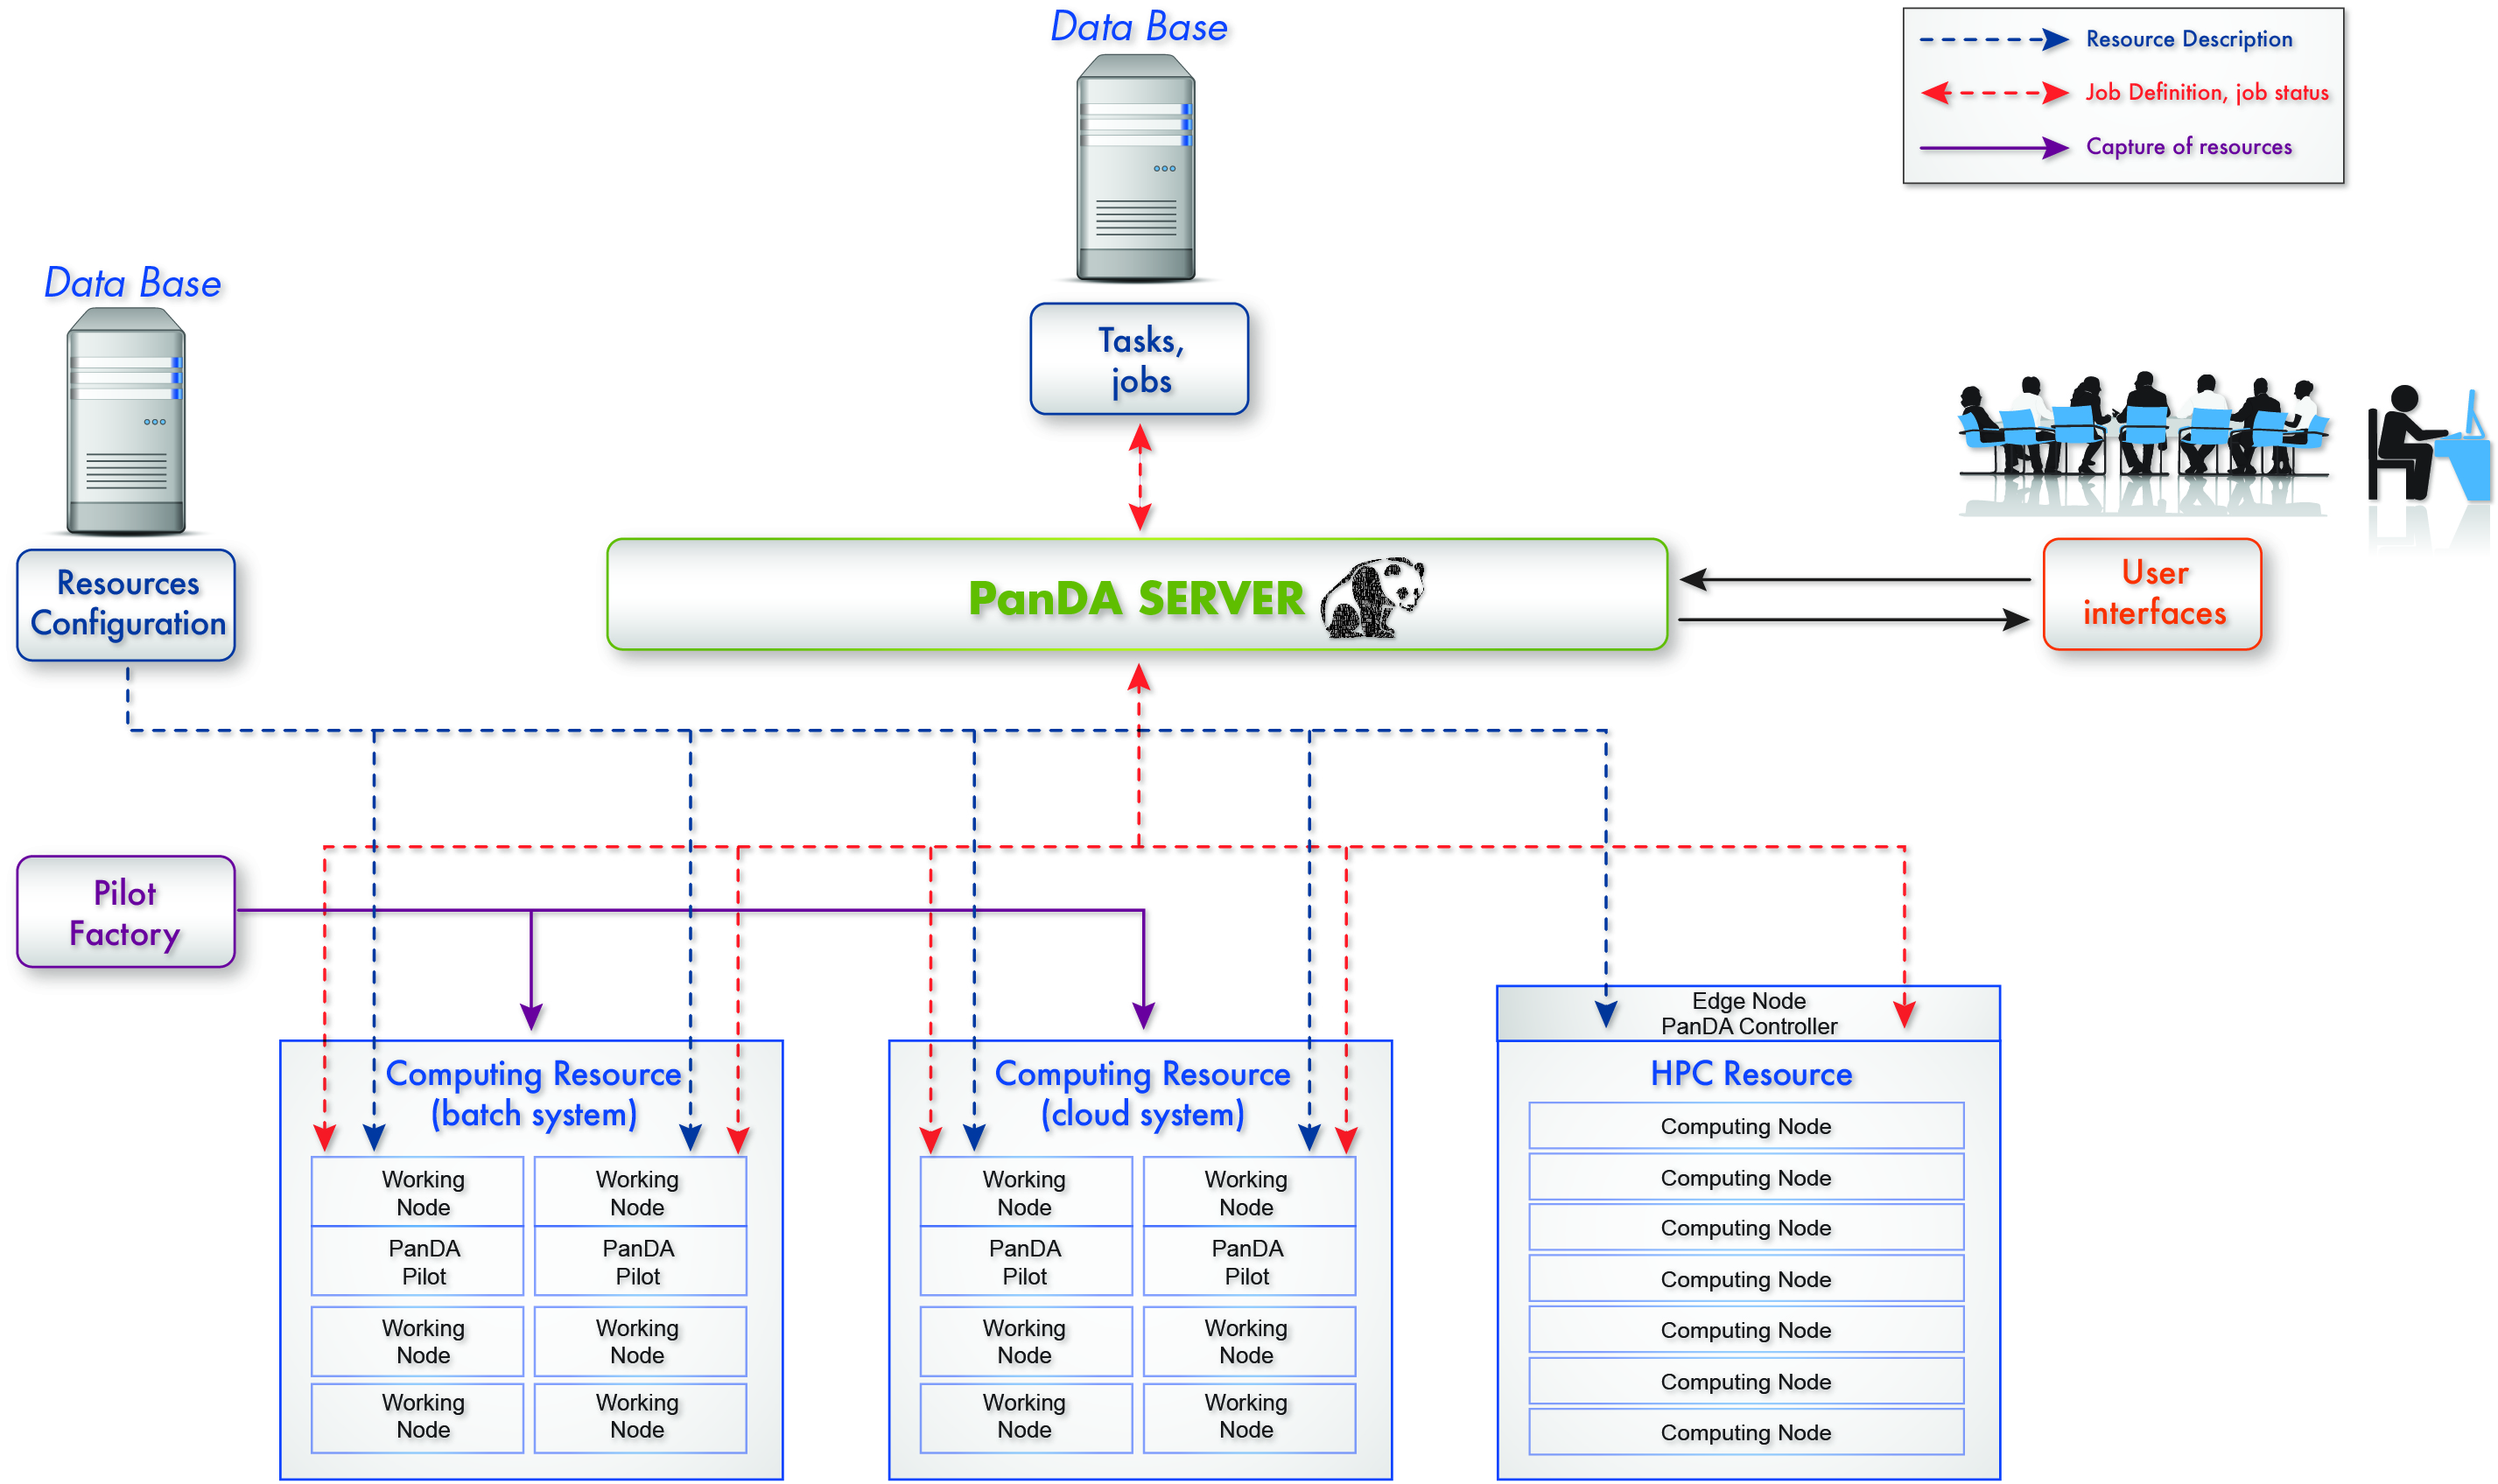
\includegraphics[width=\columnwidth]{figures/PandaArch.jpg}
  \end{center}
\caption{\mtnote{This diagram is a placeholder. I am working on a substitute
that will be referenced when describing PanDA's subsystems.}Schematic view of
the PanDA system\label{fig:architecture}, as deployed for production in 2017.
Black boxes indicate PanDA's subsystems; Orange boxes components of a subsystem;
purple boxes databases; green arrows http messaging interfaces; red arrows API;
purple arrows database communications.}
% Originally PanDA was designed for grid infrastructure... In this
% paper is focussed on the HPC use case; there are differences from
% the grid use case. This paper discusses how PanDA has been adapted
% to execute a workload % on HPC resources. The schematic overview is
% presented for workload X on Titan......
\end{figure}

\paragraph{\textbf{PanDA Server}} this subsystem is the central hub service of
PanDA and it operates as a web service. It runs on Apache web server,
interacting with the back-end database running on separate servers. It uses the
Apache worker model, with many independent  processes handling client requests
in parallel. Since all state is maintained in the central database, the PanDA
Server application instance itself is stateless. Currently production version of
PanDA utilizes Oracle database backend, but PanDA can also work with MySQL
family of databases.

% . It provides a task queue
% managing all job information centrally. The PanDA server receives jobs through
% the client interface into the task queue, upon which a brokerage module
% operates to prioritize and assign work on the basis of job type, priority,
% input data and its locality, and available CPU resources. The PanDA server

PanDA Server implementation consists of four components, all implemented in
Python and communicating via Python APIs: Task Buffer, Brokerage, Job
Dispatcher, and Data Service. Task Buffer is the management component of PanDA's
global queue and offers functionalities to: (i) store jobs into the global
queue; (ii) provide information about the state of each stored job; and (iii)
update the state of each job upon communication with the other three components
of PanDA Server. The Brokerage component enables (i) matching job attributes
with site and pilot attributes; (ii) managing the dispatch of input data to
processing sites; and (iii) deriving PanDA's data pre-placement requirement.
% The job/pilot matching algorithm assigns a weight to each candidate pilot and
% after applying a set of policies, the best ten candidates are taken.
The Job Dispatcher implements functionalities to: (i) receive requests from
active pilots for new jobs to process; (ii) retrieving from Task Buffer the jobs
with highest priority that can be executed on the resource on which the
requesting pilot has been instantiated; (iii) creating a wrapper for the
selected job, tailored to the resource of the requesting pilot; and (iv)
monitoring the state of the job execution on the pilot, updating the Task Buffer
component. Finally, the Data Service component offers functionalities to: (i)
retrieve information from Task Buffer and Brokerage about the data requirements
of each job and the resource to which each job has been assigned; (ii) enable
interaction with the ATLAS Distributed Data Management (DDM)~\cite{atlas_ddm} to
make input files available to the jobs and manage their output data.

\paragraph{\textbf{PanDA Pilot}} this subsystem is execution environment for
PanDA's jobs. Implemented in Python, a PanDA Pilot is launched by a wrapper
submitted to a target resource. Wrappers are tailored to the specific interfaces
and middleware exposed by each site so that PanDA Pilot remains
site-independent. PanDA Pilot implements four main functionalities: (i)
preparing the execution environment for PanDA's jobs, including recovering and
cleaning up previously failed jobs on that site and collecting information about
the compute, data, and network capabilities of the site; (ii) requesting a job
for execution to the Job Dispatcher component of PanDA Server; (iii) initiating
and monitoring the execution of pulled jobs, including setting up the job,
transferring its input when required, executing the payload, transferring
output, and checking log files and local space; and (iv) clean up when the
payload has finished to execute.

% PanDA is a pilot based workload management system.
% In the PanDA job lifecycle, pilot jobs (Python scripts that organize workload
% processing on a worker node) are submitted to sites. When these pilot jobs
% start on a worker node they contact a central server to retrieve a real
% payload (i.e., an end-user job) and execute it.

PanDA Pilot implements the pilot paradigm~\cite{pilot_review} and, as such, it
decouples resource acquisition from job execution via multi-stage scheduling.
This has several benefits, including increasing the number of completed jobs per
unit of resource by lowering the time taken between finishing the execution of a
job an starting a the execution of a new job; enabling both concurrent and
sequential job execution depending on the number of cores available to the pilot
and the time for which the remain available; and exposing a unified and
consistent interface for the scheduling of jobs, independent from the type of
resource on which the pilot has been instantiated and the middleware installed
on the site. The specifics implementation of PanDA Pilot enables also better
reliability by real-time monitoring of the job execution process, and a certain
degree of fault-tolerance by recovering information and, possibly, output files
from jobs that failed, even before instantiating the PanDA Pilot.

% Using these pilot-based workflows helps to improve job reliability, optimize
% resource utilization, allows for opportunistic resources usage, and mitigates
% many of the problems associated with the inhomogeneities found on the Grid.

It should be noted that upon bootstrapping, a PanDA Pilot download major parts
of its runtime code a central Subversion repository via HTTP. The repository
works with an Apache web server, configured with a memory-based web proxy
(Squid). The purpose of the cache is to reduce the request load on the
back-end Subversion server. That improves performance \mtnote{Do we have
data/numbers?} since only occasional queries trigger a full lookup on the
back-end Subversion system, and most external queries are pulled from memory
on the front-end web server. The benefits of this system include a
high-performance code download service combined with code updates still being
immediately available as soon as they are committed to source code control.

\paragraph{\textbf{AutoPyFactory}} this subsystem implements a factory to submit
pilots locally and to both grid and cloud sites. Implemented to be executed as a
single demonized process, AutoPyFactory enable the concurrent spawning of
multiple job submission processes called APFQueue. Each APFQueue can communicate
with PanDA Server and the Brokerage module to collect information about the
state of the jobs it manages and, on the base of this information, submit new
pilots to one site per APFQueue. AutoPyFactory implements functionalities to
evaluate the number of pilots already instantiated on each site, and to apply a
consistent and adequate pressure on their batch queues. Submission is performed
via the Condor-G batch system~\cite{}, enabling submission to multiple type of
sites. AutoPyFactory exposes a dedicated monitoring service, feeding information
to the PanDA Monitoring subsystem. A proxy manager is also run, enabling
certificate-based authentication and authorization.

% As a pilot-based system, PanDA requires some way to get the initial PanDA
% pilot onto worker nodes at sites. This is done with the help of a component
% called AutoPyFactory (APF). APF runs in a single daemonized process,
% launching a separate thread for each internal workflow. Each one of these
% internal workflows typically serves a single job queue as defined in WMS, and
% delivers pilots to a single batch queue, either local or remote. The behavior
% of these APF workflows is determined by the combination of a set of plugins,
% invoked in a fixed order, in a loop, each one in charge of the performance of
% a well defined action.

\paragraph{\textbf{PanDA Monitoring}} this subsystem is implemented as a
web-based, dashboard-style graphical application. It runs on Apache and
interacts with the back-end database of PanDA Server to enable persistence.
PanDA Monitoring enables users and site administrators to gather information
about the status of current and past jobs, data movement, and pilot factory.
PanDA Monitoring allows users access to all job log files on job by job basis,
greatly simplifying code debugging and failure analysis in a distributed
computing environment.

\paragraph{JEDI} \mtnote{Should we include it?}

\paragraph{Event Service} \mtnote{Should we include it?}


\subsection{Execution Process}

\mtnote{Probably move this to the workflow}
\mtnote{Think whether a comparison with other WMS based on the review we did
makes sense in this context.}

\mtnote{Summary: JEDI retrieves task descriptions and source files, converting
them into job descriptions and events sets. Jobs are submitted to PanDA Server
while events to the Event Service. The PanDA Server schedules jobs to pilots
that have been submitted to resources via the PanDA Factory. Once executed, jobs
pulls events from the Event Service as input and push output back to JEDI.}
